%%%%%%%%%%%%%%%%%%%%%%%%%%%%%%%%%%%%%%%%%%%%%%%%%%%%%%%%%%%%%%%%%%%%%%%%%%%%%%%%%%
\begin{frame}[fragile]\frametitle{}
\begin{center}
{\Large Random Forest with Scikit-Learn}

{\tiny (Ref: Ensemble Machine Learning Algorithms in Python with scikit-learn - Jason Brownlee)}
\end{center}
\end{frame}


% %%%%%%%%%%%%%%%%%%%%%%%%%%%%%%%%%%%%%%%%%%%%%%%%%%%%%%%%%%%%%%%%%%%%%%%%
% \begin{frame}[fragile]\frametitle{Random Forest Template Code}
% \begin{lstlisting}
% from sklearn.ensemble import RandomForestClassifier

% model= RandomForestClassifier() 

% model.fit(X, y) 

% predicted= model.predict(x_test) 
% \end{lstlisting}
% \end{frame}

% %%%%%%%%%%%%%%%%%%%%%%%%%%%%%%%%%%%%%%%%%%%%%%%%%%%%%%%%%%%%%%%%%%%%%%%%%%%%%%%%%%
% \begin{frame}[fragile]\frametitle{}
% \begin{center}
% {\Large Test case: Diabetes in Pima Indians}
% \end{center}
% \end{frame}

%%%%%%%%%%%%%%%%%%%%%%%%%%%%%%%%%%%%%%%%%%%%%%%%%%%%%%%%%%%
\begin{frame}[fragile]\frametitle{Random Forest Classification}

	\begin{itemize}
	\item Random forest is an extension of bagged decision trees.
	\item Samples of the training dataset are taken with replacement, but the trees are constructed in a way that reduces the correlation between individual classifiers. 
	\item Specifically, rather than greedily choosing the best split point in the construction of the tree, only a random subset of features are considered for each split.
	\end{itemize}
	
\end{frame}


%%%%%%%%%%%%%%%%%%%%%%%%%%%%%%%%%%%%%%%%%%%%%%%%%%%%%%%%%%%%%%%%%%%%%%%%
\begin{frame}[fragile]\frametitle{Random Forest Classification}
\begin{lstlisting}
# Random Forest Classification
from sklearn import model_selection
from sklearn.ensemble import RandomForestClassifier
import pandas
url = "https://archive.ics.uci.edu/ml/machine-learning-databases/pima-indians-diabetes/ pima-indians-diabetes.data"
names = ['preg', 'plas', 'pres', 'skin', 'test', 'mass', 'pedi', 'age', 'class']
dataframe = pandas.read_csv(url, names=names)
array = dataframe.values
X = array[:,0:8]
Y = array[:,8]
seed = 7
num_trees = 100
max_features = 3
kfold = model_selection.KFold(n_splits=10, random_state=seed)
model = RandomForestClassifier(n_estimators=num_trees, max_features=max_features)
results = model_selection.cross_val_score(model, X, Y, cv=kfold)
print(results.mean())

0.770727956254
\end{lstlisting}
Running the example provides a mean estimate of classification accuracy.
\end{frame}

% %%%%%%%%%%%%%%%%%%%%%%%%%%%%%%%%%%%%%%%%%%%%%%%%%%%%%%%%%%%%%%%%%%%%%%%%%%%%%%%%%%
% \begin{frame}[fragile]\frametitle{}
% \begin{center}
% {\Large Test case: Iris Flowers}
% \end{center}
% \end{frame}

% %%%%%%%%%%%%%%%%%%%%%%%%%%%%%%%%%%%%%%%%%%%%%%%%%%%%%%%%%%%%%%%%%%%%%%%%
% \begin{frame}[fragile]\frametitle{Random Forest with Iris Dataset}
% \begin{lstlisting}
% from sklearn.ensemble import RandomForestClassifier
% import pandas as pd

% train = pd.read_csv("iris_train.csv")

% test = pd.read_csv("iris_test.csv")

% print(train.head())
% \end{lstlisting}
% \begin{center}
% 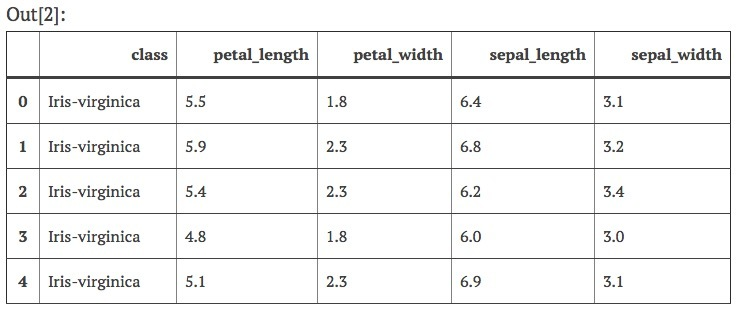
\includegraphics[width=0.5\linewidth]{iris1}
% \end{center}

% \end{frame}

% %%%%%%%%%%%%%%%%%%%%%%%%%%%%%%%%%%%%%%%%%%%%%%%%%%%%%%%%%%%%%%%%%%%%%%%%
% \begin{frame}[fragile]\frametitle{Random Forest with Iris Dataset}
% The data have to be in a numpy array in order for the random forest algorithm to accept it!
% \begin{lstlisting}
% cols = ['petal_length', 'petal_width', 'sepal_length', 'sepal_width'] 
% colsRes = ['class']

% trainArr = train.as_matrix(cols) #training array
% trainRes = train.as_matrix(colsRes) # training results

% ## Training!
% rf = RandomForestClassifier(n_estimators=100) # initialize
% rf.fit(trainArr, trainRes) # fit the data to the algorithm
% \end{lstlisting}
% \end{frame}

% %%%%%%%%%%%%%%%%%%%%%%%%%%%%%%%%%%%%%%%%%%%%%%%%%%%%%%%%%%%%%%%%%%%%%%%%
% \begin{frame}[fragile]\frametitle{Random Forest with Iris Dataset}
% Put the test data in the same format!
% \begin{lstlisting}
% testArr = test.as_matrix(cols)
% results = rf.predict(testArr)

% # something I like to do is to add it back to the data frame, so I can compare side-by-side
% test['predictions'] = results
% print(test.head())
% \end{lstlisting}
% %\begin{center}
% %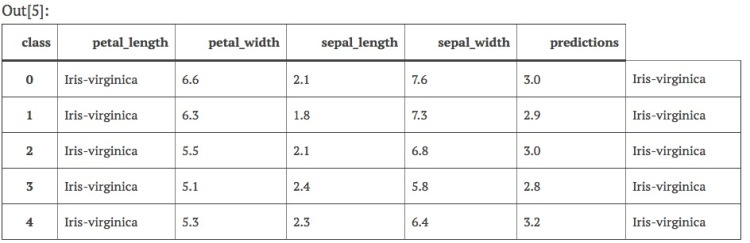
\includegraphics[width=0.5\linewidth]{iris2}
% %\end{center}
% %With this dataset, the random forest algorithm predicted class perfectly. That is unlikely to happen on a more challenging problem, but I hope now you know how to get started!
% \end{frame}

% %%%%%%%%%%%%%%%%%%%%%%%%%%%%%%%%%%%%%%%%%%%%%%%%%%%%%%%%%%
% \begin{frame}[fragile]\frametitle{Random Forests (Recap)}
% \begin{itemize}
% \item Designed for decision tree classifiers
% \item Bagging and Boosting can be applied to other learning algorithms
% \item Example of ``manipulating the input features'' 
% \item Idea: combines predictions made by multiple decision trees
% \item Each tree is induced based on an independent set of random vectors
% \item Random forests are generated from fixed probability distribution (unlike Boosting)

% \end{itemize}
% \end{frame}